\chapter{Planning et d�finition des t�ches}
\authors{
  \authorinfo{Marc}{de la Motte Rouge} \\
}

Notre projet � �t� r�alis� en une dur�e d'environ trois mois. Nous avons essay� de r�alis� un planning comprenant les diff�rentes t�ches � effectuer. Il est d�taill� sur les figures \ref{fig:gant-prevu1}, \ref{fig:gant-prevu2}, \ref{fig:gant-prevu3}. 

\begin{figure}[htpb]
  \centering
  \fbox{
    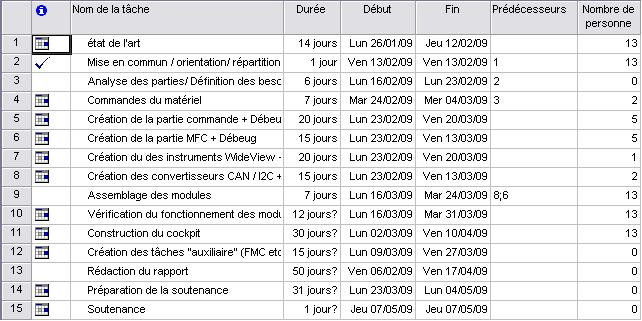
\includegraphics[scale=0.7]{images/gant_previsionnel1}
  }
  \caption{Diagramme de Gantt pr�visionnel - partie 1}
  \label{fig:gant-prevu1}
\end{figure}


\begin{figure}[htpb]
  \centering
  \fbox{
    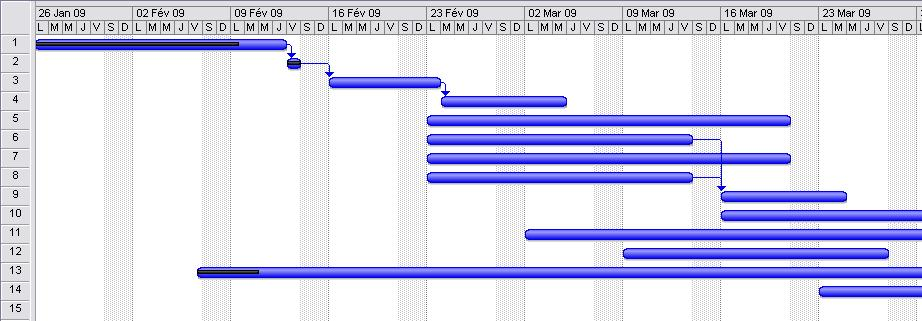
\includegraphics[scale=0.7]{images/gant_previsionnel2}
  }
  \caption{Diagramme de Gantt pr�visionnel - partie 2}
  \label{fig:gant-prevu2}
\end{figure}


\begin{figure}[htpb]
  \centering
  \fbox{
    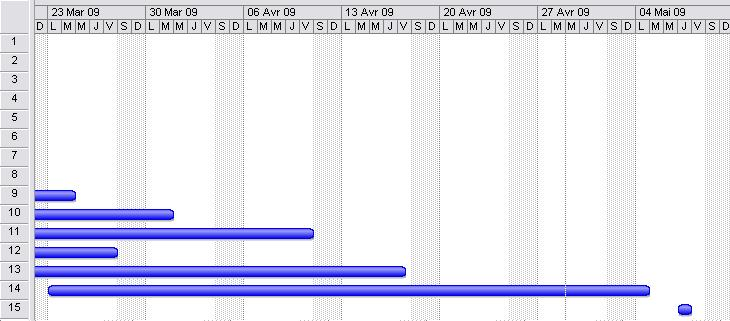
\includegraphics[scale=0.7]{images/gant_previsionnel3}
  }
  \caption{Diagramme de Gantt pr�visionnel - partie 3}
  \label{fig:gant-prevu3}
\end{figure}


Ce planning a �t� r�alis� en prenant en compte toutes les t�ches. Elles n'ont pas pu �tre toutes r�alis�es en raison de leur complexit� et du faible temps dont nous disposions. Le planning r�el suivi ainsi que les t�ches r�alis�es sont d�taill� dans les diagrammes de Gantt et Pert dans les figures \ref{fig:gant1}, \ref{fig:gant2}, \ref{fig:gant3} et \ref{fig:pert1},  \ref{fig:pert2} et  \ref{fig:pert3}.

\begin{figure}[htpb]
  \centering
  \fbox{
    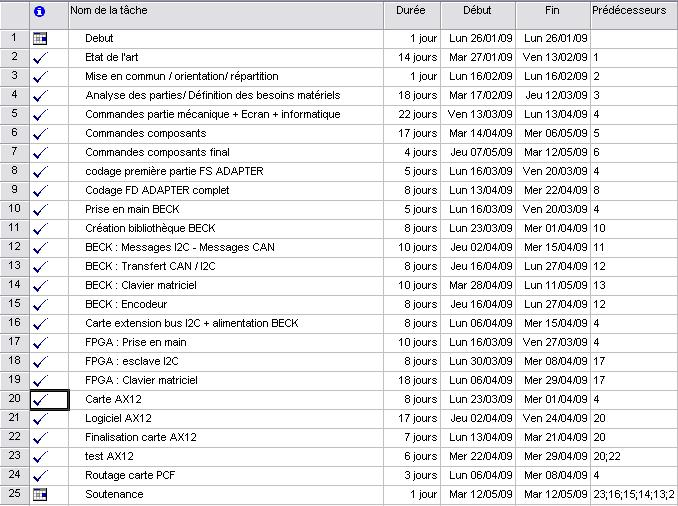
\includegraphics[scale=0.7]{images/gant1}
  }
  \caption{Diagramme de Gantt r�el - partie 1}
  \label{fig:gant1}
\end{figure}


\begin{figure}[htpb]
  \centering
  \fbox{
    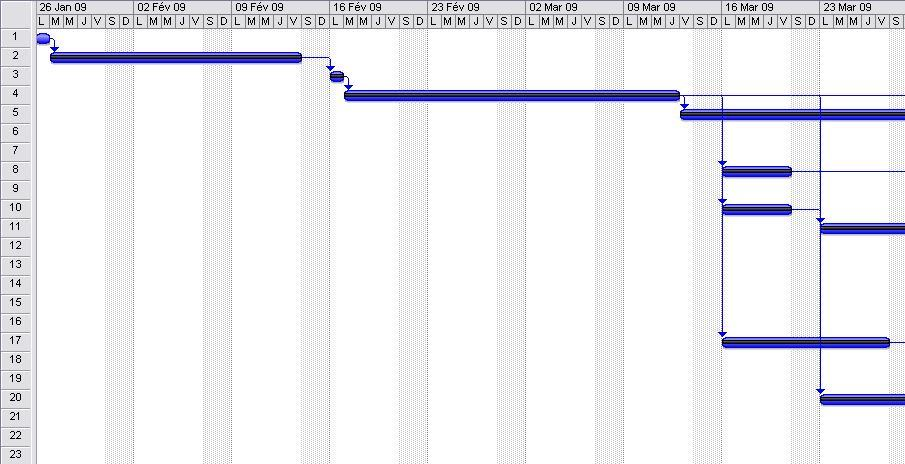
\includegraphics[scale=0.7]{images/gant2}
  }
  \caption{Diagramme de Gantt r�el - partie 2}
  \label{fig:gant2}
\end{figure}

\begin{figure}[htpb]
  \centering
  \fbox{
    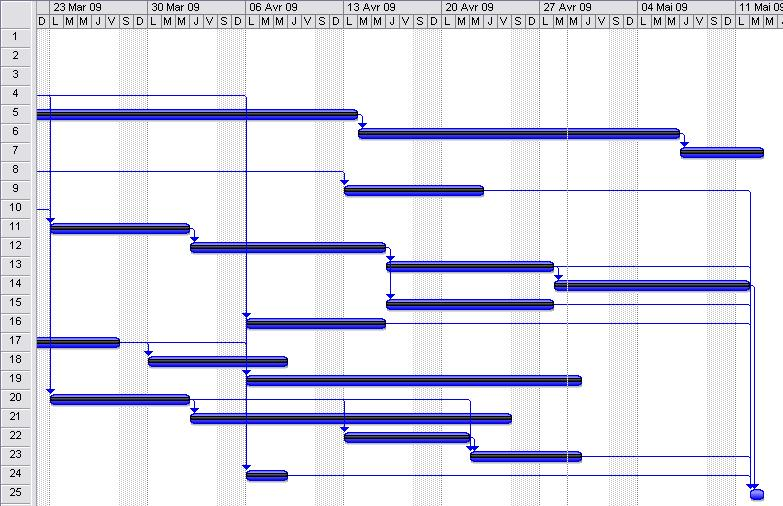
\includegraphics[scale=0.7]{images/gant3}
  }
  \caption{Diagramme de Gantt r�el - partie 3}
  \label{fig:gant3}
\end{figure}

\begin{figure}[htpb]
  \centering
  \fbox{
    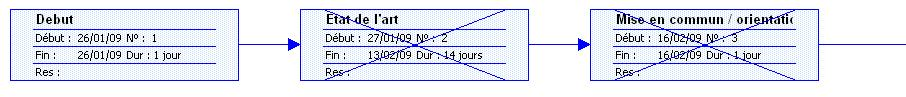
\includegraphics[scale=0.5]{images/pert1}
  }
  \caption{Diagramme de PERT r�el - partie 1}
  \label{fig:pert1}
\end{figure}

\begin{figure}[htpb]
  \centering
  \fbox{
    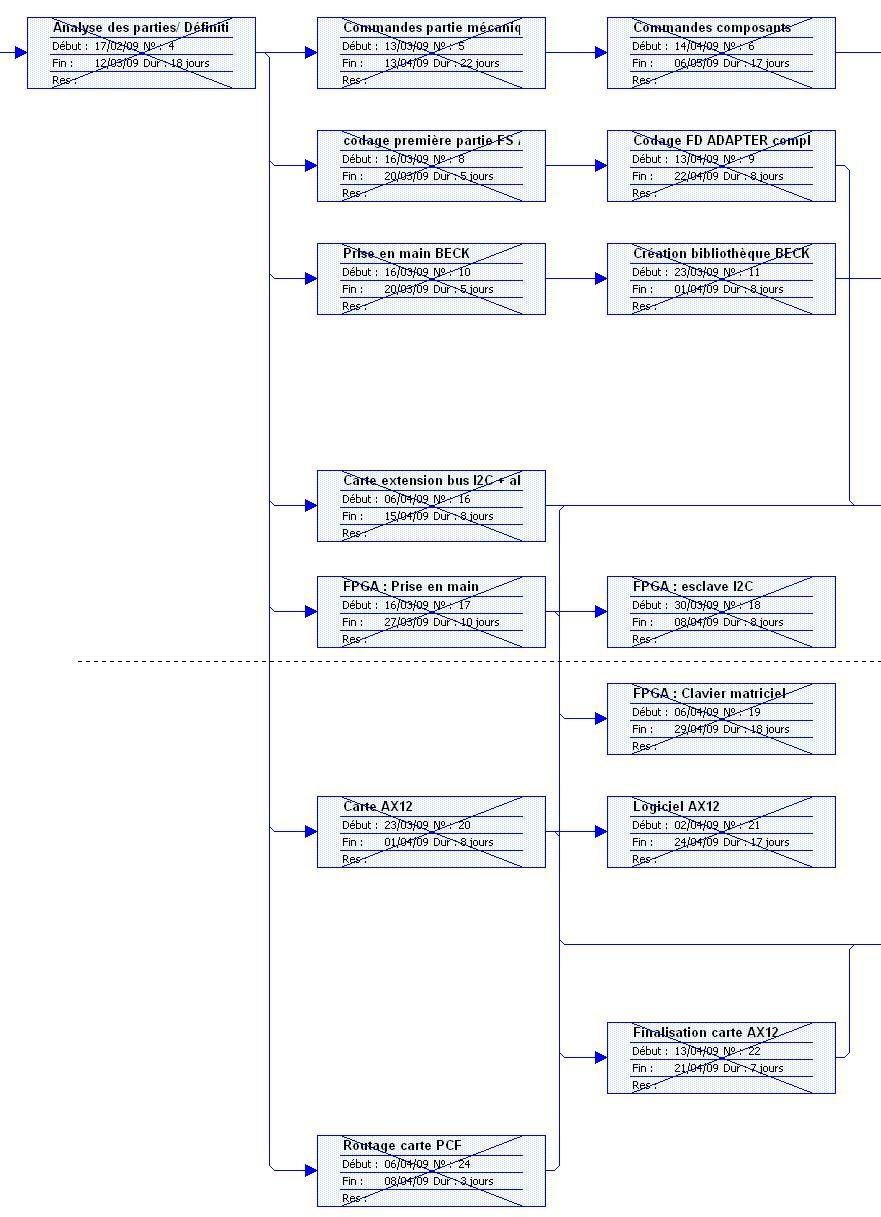
\includegraphics[scale=0.5]{images/pert2}
  }
  \caption{Diagramme de PERT r�el - partie 2}
  \label{fig:pert2}
\end{figure}

\begin{figure}[htpb]
  \centering
  \fbox{
    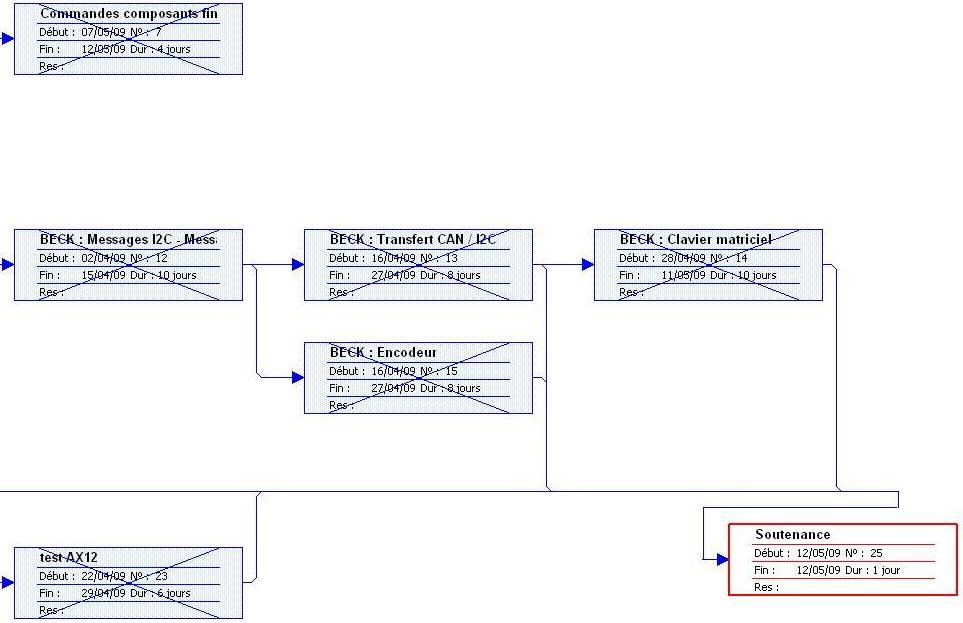
\includegraphics[scale=0.5]{images/pert3}
  }
  \caption{Diagramme de PERT r�el - partie 3}
  \label{fig:pert3}
\end{figure}